\chapter{Θετικοί και αρνητικοί αριθμοί}
\section{Θετικοί και Αρνητικοί Αριθμοί (Ρητοί αριθμοί) -
H ευθεία των ρητών - Τετμημένη σημείου}
\begin{exercise}
\sel[4]{117} 
Στα ζεύγη αριθμών που ακολουθούν να βρεις ποιοι αριθμοί είναι ομόσημοι και ποιοι είναι ετερόσημοι: (α) 3 και +3, (β) 2 και 5, (γ) –2 και –4, (δ) 7 και +9, (ε) –2 και 1,(στ) 17 και –20, (ζ) –9 και –3,2, (η) –10,5 και 11, (θ) –3 και –100, (ι) +6,7 και +12,3
\end{exercise}

Αργότερα θα μάθεις έναν εύκολο τρόπο για να ελέγξεις αν δύο αριθμοί είναι ομόσημοι οι ετερόσημοι, με όσα έχεις δει μέχρι τώρα μπορείς να το κάνεις ως εξής:
\begin{lstlisting}
    while (True):
        a = float(input('α> '))
        b = float(input('β> '))

        if a > 0:
            if b > 0:
                print("Ομόσημοι")
            else:
                print("Ετερόσημοι")
        else:
            if b < 0:
                print("Ομόσημοι")
            else:
                print("Ετερόσημοι")
\end{lstlisting}
και το αποτέλεσμα θα είναι:
\begin{lstlisting}
α>3
β>+3
Ομόσημοι
α>2
β>5
Ομόσημοι
α>-2
β>-4
Ομόσημοι
α>7
β>+9
Ομόσημοι
α>-2
β>1
Ετερόσημοι
α>17
β>-20
Ετερόσημοι
α> -9
β> -3.2
Ομόσημοι
α> -10.5
β> 11
Ετερόσημοι
α> -3
β> -100
Ομόσημοι
α> 6.7
β> 12.3
Ομόσημοι
\end{lstlisting}

\begin{exercise}
\sel[6]{117} Βρες τη λέξη που σχηματίζεται από τα γράμματα με τετμημένες –6, 10, 9, –9, 5, –5, 0 στο παρακάτω σχήμα. Στη συνέχεια γράψε μ’ αυτό τον τρόπο ένα όνομα που σου αρέσει.
Εικόνα
\end{exercise}
Οι αντιστοιχίσεις μπορούν να αποθηκευτούν σε ένα λεξικό και να βρούμε τη λέξη ως εξής:
\begin{lstlisting}
antistoixiseis = {-11:'Ψ',
-10:'Φ',
-9:'T',
-8:'Ρ',
-7:'Ξ',
-6:'Μ',
-5:'Κ',
-4:'Θ',
-3:'Ζ',
-2:'Δ',
-1:'Β',
0:'Ο',
1:'Α',
2:'Γ',
3:'Ε',
4:'Η',
5:'Ι',
6:'Λ',
7:'Ν',
8:'Π',
9:'Σ',
10:'Υ',
11:'Χ',
12:'Ω'}
tetmimenes = [-6,10,9,-9,5,-5,0]
for i in tetmimenes:
    print(antistoixiseis[i])
\end{lstlisting}

Το αποτέλεσμα θα είναι:
\begin{lstlisting}
Μ
Υ
Σ
T
Ι
Κ
Ο
\end{lstlisting}
Αν αλλάξουμε την εντολή print ως εξής:
\begin{lstlisting}
print(antistoixiseis[i],end='')
\end{lstlisting}
Θα προκύψει:
\begin{lstlisting}
ΜΥΣΤΙΚΟ
\end{lstlisting}
Με το end='' δίνουμε την οδηγία στην Python να μην αλλάζει γραμμή μετά από κάθε print.
H κωδικοποίηση γίνεται με το ίδιο λεξικό αλλά ως εξής:
\begin{lstlisting}
lexi = 'ΜΗΝΥΜΑ'
for l in lexi:
    print(list(antistoixiseis.keys())[
        list(antistoixiseis.values()).index(l)],
          end=',')
\end{lstlisting}
Ο λόγος για τον οποίο είναι τόσο πολύπλοκη η κωδικοποίηση είναι ότι το λεξικό δεν μπορεί να υποστηρίξει και τις δύο κατευθύνσεις πρόσβασης. Ένας εναλλακτικός τρόπος αναπαράστασης των ίδιων δεδομένων θα ήταν ο εξής:
\begin{lstlisting}
grammata = ['Ψ','Φ','T','Ρ','Ξ','Μ','Κ','Θ','Ζ','Δ','Β','Ο','Α','Γ','Ε','Η','Ι','Λ','Ν','Π','Σ','Υ','Χ','Ω']
arithmoi = [-11,-10,-9,-8,-7,-6,-5,-4,-3,-2,-1,0,1,2,3,4,5,6,7,8,9,10,11,12]

tetmimenes = [-6,10,9,-9,5,-5,0]
for i in tetmimenes:
    print(grammata[arithmoi.index(i)],end='')
print()

lexi = 'ΜΗΝΥΜΑ'
for l in lexi:
    print(arithmoi[grammata.index(l)],end=',')
\end{lstlisting}
που δίνει το σωστό αποτέλεσμα:
\begin{lstlisting}
ΜΥΣTΙΚΟ
-6,4,7,10,-6,1,
\end{lstlisting}
\begin{exercise}
\sel[7]{117}
Τα σημεία Α και Β έχουν τετμημένες α και β, αντίστοιχα. Να βρεθεί η τετμημένη του μέσου Μ του τμήματος ΑΒ όταν: (α) α = +5 και β = +8, (β) α = –4 και β = –13.
\end{exercise}
\begin{lstlisting}
>>> (5+8)/2
6.5
>>> (-4+(-13))/2
-8.5
\end{lstlisting}
\section{Απόλυτη τιμή}
Να συμπληρώσεις τον πίνακα που ακολουθεί:
\begin{table}[h]
\begin{tabular}{|c|c|c|c|c|c|c|}
\hline
Αριθμός& -2,73 & +7,66 & -1,05 & 0,+8,07 & -8\\\hline
Aπόσταση του σημείου που αντιστοιχεί από την αρχή του άξονα &&&&&\\\hline
\end{tabular}
\end{table}

Γνωρίζουμε ότι η απόσταση από την αρχή του άξονα είναι η απόλυτη τιμή. Η python μπορεί να υπολογίσει την απόλυτη τιμή με την ειδική εντολή abs, τα τρία πρώτα γράμματα της λέξης absolute.
Οπότε έχουμε:
\begin{lstlisting}
>>> abs(-2.73)
2.74
>>> abs(+7.66)
7.66
>>> abs(-1.05)
1.05
>>> abs(0)
0
>>> abs(+8.07)
8.07
>>> abs(-8)
8
\end{lstlisting}
\begin{exercise}
\sel[3]{121}
ΣΩΣΤΟ ή  ΛΑΘΟΣ
(α) Iσχύει η ανισότητα: $–5,7 < 5,7$. 

(β) Ισχύει η ανισότητα: $–7,6 > –6,7$. 

(γ) Στην ανισότητα $2,3 < x < 4,7$ ο x μπορεί να πάρει 2 ακέραιες τιμές. 

(δ) Υπάρχουν 5 ακριβώς ακέραιοι που αληθεύουν τη σχέση: $–2 \leq x \leq 2$.

(ε) Δύο ακέραιοι με αντίθετο πρόσημο είναι αντίθετοι.
\end{exercise}
(α)
\begin{lstlisting}
>>> -5.7 < 5.7
True
\end{lstlisting}
Σωστό
(β)
\begin{lstlisting}
>>> -7.6 > -6.7
False
\end{lstlisting}
Λάθος
(γ) 
\begin{lstlisting}
for i in range(10):
    if i > 2.3 and i < 4.7:
        print(i)
\end{lstlisting}
το αποτέλεσμα είναι:
\begin{lstlisting}
3
4
\end{lstlisting}
Ο x μπορεί να πάρει 2 ακέραιες τιμές άρα ΣΩΣΤΟ.
(δ)
\begin{lstlisting}
for i in range(-3,3):
    if i >= -2 and i <= 2:
        print(i)
\end{lstlisting}
το αποτέλεσμα είναι:
\begin{lstlisting}
-2
-1
0
1
2
\end{lstlisting}
Υπάρχουν 5 ακριβώς ακέραιοι που αληθεύουν τη σχέση άρα ΣΩΣΤΟ
(ε) Λάθος γιατί υπάρχει η εξαίρεση του μηδενός.

\begin{exercise}
\sel[4]{121} Βρες την απόλυτη τιμή των ρητών: (α) +7,25, (β) –2,5, (γ) +16, (δ) –20,05, (ε) –58.
\end{exercise}
\begin{lstlisting}
>>> abs(+7.25)
7.25
>>> abs(-2.5)
2.5
>>> abs(+16)
16
>>> abs(-20.05)
20.05
>>> abs(-58)
58
\end{lstlisting}
\begin{exercise}
\sel[5]{121}Βρες τους αριθμούς που έχουν ως απόλυτη τιμή: (α) 100, (β) 21,7, (γ) 0, (δ) 7,03, (ε) 5,2.
\end{exercise}
\begin{lstlisting}
def fromabs(x):
    if x == 0:
        return(0)
    else:
        return((x, -x))

>>> fromabs(100)
(100, -100)
>>> fromabs(21.7)
(21.7, -21.7)
>>> fromabs(0)
0
>>> fromabs(7.03)
(7.03, -7.03)
>>> fromabs(5.2)
(5.2, -5.2)
\end{lstlisting}
\begin{exercise}
\sel[6]{121}
Συμπλήρωσε τον πίνακα:
\begin{table}[h]
\begin{tabular}{|c|c|c|c|c|c|c|c|c|}
\hline
Αριθμός      &1&           &         &-19&   &    & & \\\hline
Αντίθετος    & &           &         &   & -8& 12 & & \\\hline
Απόλυτη τιμή & &\multicolumn{2}{c}{2}&   &   &    &\multicolumn{2}{c}{7}\\\hline
\end{tabular}
\end{table}
\end{exercise}
Μπορούμε να χρησιμοποιήσουμε την abs και την fromabs για να βρούμε κάποια στοιχεία του πίνακα ο οποίος διαρμορφώνεται ως εξής:
\begin{table}[h]
\begin{tabular}{|c|c|c|c|c|c|c|c|c|}
\hline
Αριθμός      &1 &   2       &    -2   &-19& 8 & -12& 7&-7\\\hline
Αντίθετος    &-1&  -2       &     2   &19 & -8& 12 &-7& 7\\\hline
Απόλυτη τιμή &1 &\multicolumn{2}{c}{2}& 19& 8 & 12 &\multicolumn{2}{c}{7}\\\hline
\end{tabular}
\end{table}

\begin{exercise}
\sel[7]{121}Toποθέτησε στον άξονα $x'Οx$ τα σημεία με τετμημένες:$–9$, $–5,5$, $+8$, $-3$, $-7,25$, $+1$, $+12$, $+3$, $+9$. 
Ποια από αυτά είναι συμμετρικά ως προς την αρχή του άξονα;
\end{exercise}
\begin{lstlisting}
import matplotlib.pyplot as plt

plt.clf()
points = [(-9,0), (-5.5,0), (8,0), (-3,0), (-7.25,0), (+1,0), (+12,0), (+3,0), (+9,0)]
pointName = ['Α','Β','Γ','Δ','Ε','Ζ','Η','Θ','Ι']
x = [p[0] for p in points]
y = [p[1] for p in points]
plt.grid()
plt.scatter(x,y, s=100 ,marker='o')
for (i,p) in enumerate(points):
    plt.annotate(pointName[i],(p[0],p[1]))

plt.show()
\end{lstlisting}
Που δίνει το αποτέλεσμα:
\begin{figure}[h]
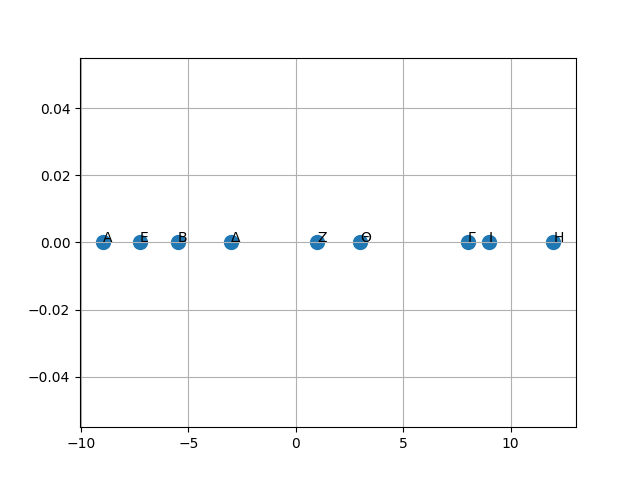
\includegraphics{graph10.png}
\end{figure}
Για να δούμε ποια είναι συμμετρικά θα πρέπει να δούμε ποια ζευγάρια έχουν τις ίδιες απόλυτες τιμές:
\begin{lstlisting}
    l = [-9, -5.5, 8, -3, -7.25, +1, +12, +3, +9]
    for i in l:
        apTimi = abs(i)
        for j in l:
            if apTimi == abs(j) and i != j:
                print(i,j)
\end{lstlisting}
Που δίνει το αποτέλεσμα:
\begin{lstlisting}
-9 9
-3 3
3 -3
9 -9
\end{lstlisting}
\begin{exercise}
\sel[8]{121}
Σχεδίασε τον άξονα $x'Ox$, με κατάλληλη μονάδα για να παραστήσεις τα σημεία με
τετμημένες τους αριθμούς: $–20,5$, $+15$, $–39,75$, $–68,25$, $+70$, $+52,25$,$+43$, $–69$.
\end{exercise}
\begin{lstlisting}
import matplotlib.pyplot as plt

plt.clf()
points = [(-20.5,0), (+15,0), (-39.75,0), (-68.25,0), (+70,0), (+52.25,0), (+43,0), (-69,0)]
pointName = ['Α','Β','Γ','Δ','Ε','Ζ','Η','Θ']
x = [p[0] for p in points]
y = [p[1] for p in points]
plt.grid()
plt.scatter(x,y, s=100 ,marker='o')
for (i,p) in enumerate(points):
    plt.annotate(pointName[i],(p[0],p[1]))

plt.show()
\end{lstlisting}
Που δίνει το αποτέλεσμα:
\begin{figure}[h]
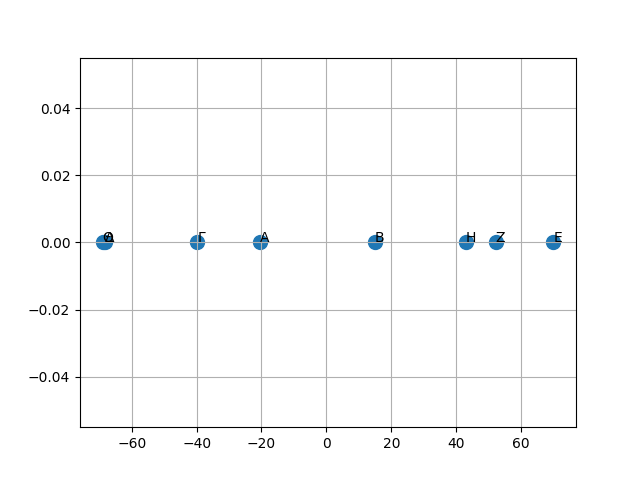
\includegraphics{graph11.png}
\end{figure}
Έτσι βλέπουμε ότι η python επέλεξε μια μονάδα να αντιστοιχεί στο 20 (1:20) και σε αυτή τη κλίμακα είναι αδύνατο να διακρίνουμε τους αριθμούς $-69$ και $-68,25$.
\begin{exercise}
Να συγκρίνεις τους αριθμούς: (α) +41 και +38, (β) 9 και 11, (γ) –3 και –2, (δ) –9 και –16, (ε) 7 και –8, (στ) 0 και –3, (ζ) 0 και +4.
\end{exercise}
\begin{lstlisting}
>>> 41 > 38
True
>>> 9 < 11
True
>>> -3 < -2
True
>>> -9 > -16
True
>>> 7 > -8
True
>>> 0 > -3
True
>>> 4 > 0
True
\end{lstlisting}
\begin{exercise}
\sel[10]{121}
Να συγκρίνεις τους αριθμούς: (α) $11$, $–11$ και $|11|$, (β) $–3$, $+3$ και $|3|$. Τι συμπεραίνεις;
\end{exercise}
\begin{lstlisting}
>>> 11 == abs(11)
True
>>> -11 < abs(11)
True
>>> -3 < abs(3)
True
>>> 3 == abs(3)
True
\end{lstlisting}
\begin{exercise}
\sel[11]{121}
Να γράψεις τους αριθμούς: –2, +7, +15, –3, 0, –4, +5, –8 και –10 σε αύξουσα σειρά.
\end{exercise}
\begin{lstlisting}
>>> print(sorted([-2, +7, +15, -3, 0, -4, +5, -8, -10]))
[-10, -8, -4, -3, -2, 0, 5, 7, 15]
\end{lstlisting}
\begin{exercise}
\sel[12]{121}
Να συμπληρώσεις με το κατάλληλο σύμβολο: <, > ή = τα κενά, ώστε να προκύψουν
αληθείς σχέσεις: (α) $–3 \ldots –8$, (β) $–4 \ldots 10$, (γ) $0 \ldots –1$, (δ) $+3 \ldots 0$, (ε) $–5 \ldots –|–5|$,
(στ) $–5 \ldots –(+5)$, (ζ) $|+7| \ldots |–7|$, (η) $–(–8) \ldots –8$, (θ) $+3 \ldots –(+4)$, (ι) $0 \ldots –|–4|$.
\end{exercise}
\begin{lstlisting}
>>> -3 > -8
True
>>> -4 < 10
True
>>> 0 > -1
True
>>> 3 > 0
True
>>> -5 == -abs(-5)
True
>>> -5 == -(+5)
True
>>> abs(+7) == abs(-7)
True
>>> -(-8) > -8
True
>>> 3 > -(+4)
True
>>> 0 > -abs(-4)
True
\end{lstlisting}

\begin{exercise}
Το x παριστάνει έναν ακέραιο αριθμό. Για ποιες τιμές του x θα ισχύουν οι σχέσεις:
(α) $–13 < x < –8$, (β) $–4 > x > –5$, (γ) $–2 < x < 5$.
\end{exercise}
\begin{lstlisting}
>>> for i in range(-14,-7):
    if i > -13 and i < -8:
        print(i) 
-12
-11
-10
-9
>>> for i in range(-6,0):
    if i < -4 and i > -5:
        print(i) 

>>> for i in range(-3,6):
    if i>-2 and i<5:
        print(i)
-1
0
1
2
3
4
\end{lstlisting}
\section{Πρόσθεση ρητών αριθμών}
\begin{exercise}
\sel[1]{123}
Σε μια πόλη παρατηρήθηκαν οι παρακάτω αυξομειώσεις της θερμοκρασίας:
Αρχικές θερμοκρασίες Αυξομειώσεις θερμοκρασίας

(α) Βράδυ +1°C την επόμενη μέρα αυξήθηκε κατά 4°C

(β) Μεσημέρι –1°C το βράδυ μειώθηκε κατά 2°C

(γ) Βράδυ –2°C την επόμενη μέρα αυξήθηκε κατά 5°C

(δ) Μεσημέρι +5°C το βράδυ μειώθηκε κατά 7°C

(ε) Μεσημέρι –3°C το βράδυ μειώθηκε κατά 3°C
\end{exercise}
\begin{lstlisting}
>>> 1 + 4
5
>>> -1 + (-2)
-3
>>> -2 + 5
3
>>> 5 + (-7)
-2
>>> +3 + (-3)
0
\end{lstlisting}
\begin{exercise}
\sel[2]{124}
Να υπολογιστούν τα παρακάτω αθροίσματα:
(α) $(+5,6) + (+8,7) + (-3,2) + (-6,9) + (+3,2) + (-7,4)$ και
(β) $(-1,8) + (+4,8) + (+9,7) + (-4,8) + (-3,4) + (+1,5)$.
\end{exercise}
\begin{lstlisting}
>>> (+5.6) + (+8.7) + (-3.2) + (-6.9) + (+3.2) + (-7.4)
-2.6645352591003757e-15
\end{lstlisting}
Στην ουσία το αποτέλεσμα είναι 0, αυτός ο αριθμός είναι πολύ μικρός.
\begin{lstlisting}
>>> (-1.8) + (+4.8) + (+9.7) + (-4.8) + (-3.4) + (+1.5)
6.0
\end{lstlisting}

\begin{exercise}
\sel[2]{125}
Υπολόγισε τα αθροίσματα:
(α) (+4,05) + (+6,15), 

(β) (+5,03) + (+4,07), 

(γ) (+2,7) + (+97,3),

(δ) (+2,6) + (+11,4), 

(ε) (+7,25) + (+8,75), 

(στ) (–3,5) + (–2,5),

(ζ) (–1,3) + (–5,2), 

(η) (–7,15) + (–4,85), 

(θ) (–5,25) + (–9,75), 

(ι) (–13,7) + (–6,3).
\end{exercise}
\begin{lstlisting}
>>> (+4.05) + (+6.15)
10.2
>>> (+5.03) + (+4.07)
9.100000000000001
>>> (+2.7) + (+97.3)
100.0
>>> (+2.6) + (+11.4)
14.0
>>> (+7.25) + (+8.75)
16.0
>>> (-3.5) + (-2.5)
-6.0
>>> (-1.3) + (-5.2)
-6.5
>>> (-7.15) + (-4.85)
-12.0
>>> (-5.25) + (-9.75)
-15.0
>>> (-13.7) + (-6.3)
-20.0
>>>
\end{lstlisting}
\begin{exercise}
Υπολόγισε τα αθροίσματα:
(α) $(+4,05) + (–6,15)$, 

(β) $(+5,03) + (–4,07)$, 

(γ) $(–2,7) + (+97,3)$,

(δ) $(–2,6) + (+11,4)$, 

(ε) $(+7,25) + (–8,75)$, 

(στ)$ (+3,5) + (–2,5)$,

(ζ) $(–1,3) + (+5,2)$,

(η) $(+7,15) + (–4,85)$, 

(θ) $(–5,25) + (+9,75)$, 

(ι) $(+13,7) + (–6,3)$.
\end{exercise}
\begin{lstlisting}
>>> (+4.05) + (-6.15)
-2.1000000000000005
>>> (+5.03) + (-4.07)
0.96
>>> (-2.7) + (+97.3)
94.6
>>> (-2.6) + (+11.4)
8.8
>>> (+7.25) + (-8.75)
-1.5
>>> (+3.5) + (-2.5)
1.0
>>> (-1.3) + (+5.2)
3.9000000000000004
>>> (+7.15) + (-4.85)
2.3000000000000007
>>> (-5.25) + (+9.75)
4.5
>>> (+13.7) + (-6.3)
7.3999999999999995
\end{lstlisting}
\begin{exercise}
\sel[4]{125}
\begin{table}[h]
\begin{tabular}{|c|c|c|c|c|}
\hline
+&+4&-8&-11&+17\\\hline
-5& &  &   &   \\\hline
+9& &  &   &   \\\hline
-4& &  &   &   \\\hline
-21&&  &   &   \\\hline
\end{tabular}
\end{table}
\end{exercise}
\begin{lstlisting}
>>> for i in [+4,-8,-11,+17]:
    for j in [-5,+9,-4,-21]:
        print(i,'+',j,'=',i+j)
4 + -5 = -1
4 + 9 = 13
4 + -4 = 0
4 + -21 = -17
-8 + -5 = -13
-8 + 9 = 1
-8 + -4 = -12
-8 + -21 = -29
-11 + -5 = -16
-11 + 9 = -2
-11 + -4 = -15
-11 + -21 = -32
17 + -5 = 12
17 + 9 = 26
17 + -4 = 13
17 + -21 = -4        
\end{lstlisting}
και ο πίνακας γίνεται:
\begin{table}[h]
\begin{tabular}{|c|c|c|c|c|}
\hline
+ &  +4&-8 &-11&+17\\\hline
-5&  -1&-13&-16& 12\\\hline
+9&  13&1  & -2& 26\\\hline
-4&   0&-12&-15& 13\\\hline
-21&-17&-29&-32& -4\\\hline
\end{tabular}
\end{table}
\begin{exercise}
\sel[5]{125}
Toποθέτησε στα κενά τα κατάλληλα πρόσημα, ώστε να προκύψουν αληθείς ισότητες:

(α) $(\ldots 6) + (-8) = -2$, 

(β) $(+5) + (\ldots 5) = 0$, 

(γ) $(+7) + (\ldots 9) = +16$,

(δ) $(\ldots 9) + (\ldots 8) = –17$, 

(ε) $(\ldots 6) + (\ldots 5) = +11$.

\end{exercise}
\begin{lstlisting}
>>> +6 + (-8) == -2
True
>>> (+5) + (-5) == 0
True
>>> (+7) + (+9) == 16
True
>>> (-9) + (-8) == -17
True
>>> (+6) + (+5) == +11
True
\end{lstlisting}
\begin{exercise}
\sel[6]{125}
Εξέτασε αν είναι μαγικά τα τετράγωνα:
(Μαγικά τετράγωνα είναι αυτά στα οποία
η πρόσθεση των αριθμών κάθε στήλης ή
γραμμής, καθώς και των διαγωνίων
τους, δίνουν το ίδιο ακριβώς άθροισμα).
\begin{table}[h]
\begin{tabular}{|c|c|c|}
\hline
-1&+4&-3\\\hline
-2&0&+2\\\hline
+3&-4&+1\\\hline
\end{tabular}
\end{table}
\begin{table}[h]
\begin{tabular}{|c|c|c|}
\hline
+1,1&+2,4&-2,5\\\hline
-0,1&+3,5&-2,4\\\hline
0&-4,9&+5,9\\\hline
\end{tabular}
\end{table}
\end{exercise}
Ένα τετράγωνο με αριθμούς μπορεί να απαρασταθεί σαν μια λίστα από λίστες ως εξής:
\begin{lstlisting}
a = [[-1,+4,-3],
        [-2,0,+2],
        [+3,-4,+1]]
b = [[+1.1,+2.4,-2.5],
         [-0.1,+3.5,-2.4],
         [0,-4.9,+5.9]]
\end{lstlisting}
Κάθε στοιχείο της λίστας a είναι μια λίστα με κάθε γραμμή του πίνακα οπότε για να βρούμε αν όλες οι γραμμές έχουν το ίδιο άθροισμα θα πρέπει να βρούμε το πρώτο και να συγκρίνουμε τις υπόλοιπες με αυτό.
\begin{lstlisting}
def ismagic(s):
    athrElegxou = s[0][0]+s[0][1]+s[0][2]
    for i in  range(3):
        athr = s[i][0]+s[i][1]+s[i][2]
        if athr!= athrElegxou:
            return(False)
    return(True)
\end{lstlisting}
Το παραπάνω πρόγραμμα ελέγχει μόνο τις γραμμές  θα πρέπει να ελέγξουμε και τις στήλες οι στήλες είναι οι εξής:
\begin{lstlisting}
>>> a[0][0]
-1
>>> a[1][0]
-2
>>> a[2][0]
3
\end{lstlisting}
Έτσι το πρόγραμμα διαμορφώνεται ως εξής:
\begin{lstlisting}
def ismagic(s):
    athrElegxou = s[0][0]+s[0][1]+s[0][2]
    for i in  range(3):
        athr = s[i][0]+s[i][1]+s[i][2]
        if athr!= athrElegxou:
            return(False)
    for i in range(3):
        athr = s[0][i] + s[1][i]+s[2][i]
        if athr!=athrElegxou:
            return(False)
    return(True)
    \end{lstlisting}
Τέλος πρέπει να ελέγξουμε τις διαγωνίους που είναι οι \lstinline{a[0][0],a[1][1],a[2][2]} και \lstinline{a[0][2],a[1][1],a[2][0]}. Οπότε το τελικό πρόγραμμα γίνεται:
 \begin{lstlisting}
def ismagic(s):
    athrElegxou = s[0][0]+s[0][1]+s[0][2]
    for i in  range(3):
        athr = s[i][0]+s[i][1]+s[i][2]
        if athr!= athrElegxou:
            return(False)
    for i in range(3):
        athr = s[0][i] + s[1][i]+s[2][i]
        if athr!=athrElegxou:
            return(False)
    athr = a[0][0]+a[1][1]+a[2][2]
    if athr!=athrElegxou:
        return(False)
    athr = a[0][2]+a[1][1]+a[2][0]
    if athr!=athrElegxou:
        return(False)
    return(True)
\end{lstlisting}
Εκτελώντας την παραπάνω συνάρτηση παίρνουμε:
\begin{lstlisting}
>>> ismagic(a)
True
>>> ismagic(b)
False
\end{lstlisting}
Που σημαίνει ότι ο πρώτος πίνακας είναι μαγικό τετράγωνο ενώ ο δεύτερος δεν είναι. Όντως για τον δεύτερο βλέπουμε στις διαγώνιες ότι:
\begin{lstlisting}
>>> +1.1+3.5+5.9
10.5
>>> -2.5+3.5+0
1
\end{lstlisting}

\begin{exercise} \sel[7]{125} Υπολόγισε τα αθροίσματα:
(α) $(-3.8)+(+2.8)+(-5.4)+(+8.2)$

(β) $(-3.5)+(-9.99)+(+2.5)+(-15.75)+(+20.75)+(+9.99)$

\end{exercise}
\begin{lstlisting}
>>> (-3.8)+(+2.8)+(-5.4)+(+8.2)
1.799999999999999
>>> (-3.5)+(-9.99)+(+2.5)+(-15.75)+(+20.75)+(+9.99)
3.9999999999999982
\end{lstlisting}

\begin{exercise}
\sel[8]{125}
Υπολόγισε τα αθροίσματα:
(α) $\left(+\frac{9}{4}\right)+\left(-\frac{5}{4}\right)+\left(\frac{2}{3}\right)+\left(-\frac{5}{3}\right)+\left(\frac{7}{13}\right)+\left(-\frac{20}{13}\right)$ και 

(β) $\left(+\frac{1}{7}\right)+\left(-\frac{5}{7}\right)+\left(+\frac{3}{5}\right)+\left(-\frac{1}{35}\right)$
\end{exercise}
\begin{lstlisting}
>>> from fractions import Fraction
>>> (+Fraction(9,4))+(-Fraction(5,4))+(Fraction(2,3))+(-Fraction(5,3))+(Fraction(7,13))+(-Fraction(20,13))
Fraction(-1, 1)
>>> (+Fraction(1,7))+(-Fraction(5,7))+(+Fraction(3,5))+(-Fraction(1,35))
Fraction(0, 1)
\end{lstlisting}
Οπότε οι απαντήσεις είναι -1 και 0 αντίστοιχα.
\section{Αφαίρεη ρητών αριθμών}
\begin{exercise}
\sel[1]{127} Ένα βράδυ το θερμόμετρο στο μπαλκόνι ενός σπιτιού έδειχνε -3$^o$C και μέσα στο σπίτι 18$^o$C. Πόση ήταν η διαφορά θερμοκρασίας;
\end{exercise}
\begin{lstlisting}
>>> 18 - (-3)
21
\end{lstlisting}
\begin{exercise}
\sel[2]{127}
Ένας έμπορος χρωστάει στον προμηθευτή του 897,56€ και του οφείλει ένα πελάτης 527,42€. Πόσα € πρέπει να έχει στο ταμείο για να ξεχρεώσει;
\end{exercise}
\begin{lstlisting}
>>> (+897.56)-(+527.42)
370,14
\end{lstlisting}
\begin{exercise}
\sel[3]{127} Να λυθούν οι εξισώσεις:

(α) $x+(+3)=(-9)$ 

(β) $(-8)-x=+7$
\end{exercise}
\begin{lstlisting}
>>> from sympy import symbols,solve
>>> x = symbols('x')
>>> expr=x+(+3)+(+9)
>>> solve(expr)
[-12]
>>> expr=(-8)-x-7
>>> solve(expr)
[-15]
\end{lstlisting}

\begin{exercise}
\sel[4]{127}
Να βρεθεί η τιμή της παράστασης $-13-(0,38-11-13)+(0,38-11)$.
\end{exercise}
\begin{lstlisting}
>>> -13-(0.38-11-13)+(0.38-11)
-1.7763568394002505e-15
>>> 
\end{lstlisting}
Στην ουσία η απάντηση είναι 0.
\begin{exercise}
\sel[1]{128} 
δ) Ισχύει  ότι:    $ 6 - ( + 8 ) + ( + 5 ) + ( - 3 ) + ( 2 ) + ( - 1 ) = 0 $ .

ε) Λύση    της εξίσωσης    $x+(-3) = -2$  είναι   ο   αριθμός $+1$.   

στ) Οι  εξισώσεις  $x+(-2)=+5$   και $x-(+7)=10+(+5)$ έχουν   την
         ίδια   λύση.
ζ) Λύση της εξίσωσης    $x- (-2)$    = $-8  +   (+7) - (-4)$    είναι   ο   αριθμός $+1$.
\end{exercise}
δ)
\begin{lstlisting}
>>> 6 - ( + 8 ) + ( + 5 ) + ( - 3 ) + ( 2 ) + ( - 1 ) == 0
False
>>> 6 - ( + 8 ) + ( + 5 ) + ( - 3 ) + ( 2 ) + ( - 1 )
1
\end{lstlisting}
Άρα λάθος
ε) Στην python μπορούμε να δούμε αν η λύση της μιας εξίσωσης είναι ένας αριθμός λύνοντάς τη ή αντικαθιστώντας τη λύση και βλέποντας αν ισχύει.
\begin{lstlisting}
from sympy import symbols,solve
>>> x = symbols('x')
>>> expr = x+(-3)
>>> expr.subs(x,1)
-2
>>> expr = expr + 2
>>> expr
x-1
>>> solve(expr)
[1]
\end{lstlisting}
στ) 
\begin{lstlisting}
>>> from sympy import symbols,solve
>>> x = symbols('x')
>>> expr1 = x+(-2)-(+5)
>>> solve(expr1)
7
>>> expr2 = x-(+7)-(10+(+5))
>>> solve(expr2)
22
\end{lstlisting}
Άρα Λάθος
ζ)
\begin{lstlisting}
>>> from sympy import symbols,solve
>>> x = symbols('x')
>>> expr = x-(-2)-(-8 +(+7)-(-4))
>>> solve(expr)
[1]
\end{lstlisting}
Δεύτερη λύση:
\begin{lstlisting}
>>> expr = x-(-2)
>>> expr.subs(x,1) == -8 +(+7)-(-4)
True
\end{lstlisting}
Άρα Σωστό
\begin{exercise}
Υπολόγισε   τις διαφορές:
(α) $5-(-7)$,   (β) $-8-(+8)$,   (γ) $-2-(-15,2)$,    (δ) $14,55-18,45$,  (ε) $-\frac{2}{7} - \left(-\frac{2}{7} \right)$.
\end{exercise}
\begin{lstlisting}
from fractions import Fraction
>>> 5-(-7)
12
>>> -8-(+8)
-16
>>> -2-(-15.2)
13.2
>>> 14.55-18.45
-3.8999999999999986
>>> -Fraction(2,7)-(-Fraction(2,7))
Fraction(0, 1)
>>>
\end{lstlisting}
\begin{exercise}
\sel[3]{128}
Κάνε    τις πράξεις:
(α) $|+3|    +   |-2|    +   |-9|$,       (β) $|-20|   +   |-10| - |+10|$,          (γ) $|-3| - |-2|+ |-5| - |+6|$.
\end{exercise}
\begin{lstlisting}
>>> abs(+3)+abs(-2)+abs(-9)
14
>>> abs(-20)+abs(-10)-abs(+10)
20
>>> abs(-3)-abs(-2)+abs(-5)-abs(+6)
0
\end{lstlisting}
\begin{exercise}
\sel[4]{128}Κάνε    τις πράξεις:
(α) $(+5) - (+3) +   (+8)$,       (β) $(-25)   +   (-4)    -   (-10)$,      (γ) $(+12)   +   (+2)    -   (-8)$.
\end{exercise}
\begin{lstlisting}
>>> (-25)+(-4)-(-10)
-19
>>> (+12)+(+2)-(-8)
22
>>>
\end{lstlisting}
\begin{exercise}
\sel[5]{128}
Συμπλήρωσε  τον πίνακα  με  τους
κατάλληλους αριθμούς:       
\begin{table}{h}
\begin{tabular}{|c|c|c|c|}
\hline
$\alpha$&$\beta$&$\alpha+\beta$&$\alpha-\beta$\\\hline
+3&&-5&\\\hline
&-8&10&\\\hline
-2&-5&&\\\hline
-9&&+6&\\\hline
\end{tabular}
\end{table}
\end{exercise}
\begin{lstlisting}
>>> from sympy import symbols,solve
>>> a = symbols('a')
>>> b = symbols('b')
>>> solve(3+b-(-5))
[-8]
>>> b = -8
>>> a = 3
>>> a-b
11
>>> solve(a-8-10)
[18]
>>> b = -8
>>> a =  18
>>> a - b
26
>>> -2+(-5)
-7
>>> -2 -(-5)
3
>>> solve(-9+b-6)
[15]
>>> a = -9
>>> b = 15
>>> a - b
-24
\end{lstlisting}

Και ο πίνακας γίνεται:
\begin{table}{h}
\begin{tabular}{|c|c|c|c|}
\hline
$\alpha$&$\beta$&$\alpha+\beta$&$\alpha-\beta$\\\hline
+3&-8&-5&11\\\hline
18&-8&10&26\\\hline
-2&-5&-7&3\\\hline
-9&15&+6&-24\\\hline
\end{tabular}
\end{table}
\begin{exercise}
\sel[5]{128}
Να  λύσεις  τις εξισώσεις:  (α) $x+(-8) = -18$, 
(β) $x + 12 = -14$,
(γ) $x+ \frac{5}{4} = \frac{7}{8}$
(δ) $x- \frac{5}{4} = 2$
\end{exercise}
\begin{lstlisting}
from sympy import symbols, solve
from fractions import Fraction
expr = x+(-18) -(-18)
solve(expr)
expr = x+12-(-14)
solve(expr)
expr = x+Fraction(5,4) - Fraction(7,8)
solve(expr)
expr  = x - Fraction(5,4) - 2
solve(expr) >>> from sympy import symbols, solve
>>> from fractions import Fraction
>>> expr = x+(-18) -(-18)
>>> solve(expr)
0
>>> expr = x+12-(-14)
>>> solve(expr)
-26
>>> expr = x+Fraction(5,4) - Fraction(7,8)
>>> solve(expr)
\end{lstlisting}
$$\frac{-3}{8}$$
\begin{lstlisting}
>>> expr  = x - Fraction(5,4) - 2
>>> solve(expr)
\end{lstlisting}
$$\frac{13}{4}$$
\begin{exercise}
\sel[7]{128}
Συμπλήρωσε  τις δύο τελευταίες  στήλες  του πίνακα:
Τι   συμπεραίνεις    για     τους    αριθμούς    των     δύο     αυτών  
στηλών;
\begin{table}[h]
\begin{tabular}{|c|c|c|c|}
$\alpha$&$\beta$&$\alpha-\beta$&$\beta-\alpha$\\\hline
$7$&$3$&&\\\hline
$2\frac{3}{4}$&$3\frac{1}{4}$&&\\\hline
$-5.55$&$-2.45$&&\\\hline
$3$&-2.1&&\\\hline
\end{tabular}
\end{table}
\end{exercise}
\begin{lstlisting}
from fractions import Fraction
al = [7,2+Fraction(3,4),-5.55,3]
bl = [3,3+Fraction(1,5),-2.45,-2.1]
for i in range(4):
    a=al[i]
    b=bl[i]
    print(a+b)
    print(a-b)
\end{lstlisting}
και το αποτέλεσμα είναι:
\begin{lstlisting}
4
-4
-9/20
9/20
-3.0999999999999996
3.0999999999999996
5.1
-5.1
\end{lstlisting}
\begin{exercise}
\sel[8]{128}
Υπολόγισε   την τιμή    των παραστάσεων με  δύο τρόπους:    
(α) $11-(12-2)+(10-5)-(8+5)$, 
(β) $-(13,7-2,6)+14,8-(-8,7+5)$,  
(γ)  $\frac{1}{6} -\left(\frac{3}{4} - \frac{5}{4}\right) - \left(\frac{7}{12}+\frac{5}{6}\right)$
\end{exercise}
\begin{lstlisting}
>>> from fractions import Fraction
>>> 11-(12-2)+(10-5)-(8+5)
-7
>>> -(13.7-2.6)+14.8-(-8.7+5)
7.4
>>> Fraction(1,6) -(Fraction(3,4) - Fraction(5,4)) - (Fraction(7,12)+Fraction(5,6))
Fraction(-3, 4)
>>>
\end{lstlisting}
\begin{exercise}
\sel[9]{128}
Συμπλήρωσε  τον πίνακα: 
\begin{table}[h]
\begin{tabular}{|c|c|c|c|c|}
x&$3,5$&&$1,89$&$-\frac{1}{4}$\\\hline
y&$-1,5$&$4,3$&&$-\frac{1}{4}$\\\hline
z&&$$-2,3$$&$3,11$&\\\hline
x+y+z&$0$&&$0,22$&$\frac{1}{2}$\\\hline
x-y-z&&0&&\\\hline
\end{tabular}
\end{table}
\end{exercise}
\begin{lstlisting}
>>> from sympy import symbols,solve
>>> from fractions import Fraction
>>> x,y,z = symbols('x y z')
>>> x = 3.5
>>> y = -1.5
>>> solve(x+y+z,z)
[-2.00000000000000]
>>> z = -2
>>> x-y-z
7.0
>>> y = 4.3
>>> z = -2.3
>>> x,y,z = symbols('x y z')
>>> y = 4.3
>>> z = -2.3
>>> solve(x-y-z,x)
[2.00000000000000]
>>> x = 2
>>> x + y + z
4.0
>>> x,y,z = symbols('x y z')
>>> x = 1.89
>>> z = 3.11
>>> solve(x+y+z-0.22,y)
[-4.78000000000000]
>>> y = -4.78
>>> x -y -z
3.56
>>> x,y,z = symbols('x y z')
>>> x = -Fraction(1,4)
>>> y = -Fraction(1,4)
>>> solve(x+y+z-Fraction(1,2),z)
[1]
>>> z = 1
>>> x-y-z
Fraction(-1, 1)
>>>
\end{lstlisting}
και ο πίνακας γίνεται:
\begin{table}[h]
\begin{tabular}{|c|c|c|c|c|}
x&$3,5$&$2$    &$1,89$&$-\frac{1}{4}$\\\hline
y&$-1,5$&$4,3$&$-4.7$8&$-\frac{1}{4}$\\\hline
z&$-2$&$-2,3$&$3,11$&1\\\hline
x+y+z&$0$&4&$0,22$&$\frac{1}{2}$\\\hline
x-y-z&7&0&3.56&-1\\\hline
\end{tabular}
\end{table}
\section{Πολλαπλασιασμός ρητών αριθμών}
\begin{exercise}
\sel[1]{131}
Nα	υπολογιστούν	τα	γινόμενα:	(α)	$(–1,4)\cdot 5$,		(β)	$\left(+ \frac{2}{3}\right)\cdot(–2,1)$,			(γ)	$(–10)\cdot(–0,7)$.
\end{exercise}
\begin{lstlisting}
>>> from fractions import Fraction
>>> -1.4*5
-7.0
>>> (+Fraction(2,3))*(-2.1)
-1.4
>>> (-10)*(-0.7)
7.0
>>>
\end{lstlisting}
\begin{exercise}
\sel[2]{131}
Nα	υπολογιστεί	το	γινόμενο	$(–1)\cdot α$,	όταν	το	α	παίρνει	τις	τιμές:$+3$,	$–1,2$,	$+\frac{2}{3}$, $-2$.
\end{exercise}
\begin{lstlisting}
from fractions import Fraction
al = [+3,-1.2,+Fraction(2,3),-2]
for a in al:
    print(-1*a)
\end{lstlisting}
που δίνει το αποτέλεσμα:
\begin{lstlisting}
-3
1.2
-2/3
2
\end{lstlisting}
\begin{exercise}
\sel[4]{131}
Να	υπολογιστεί	η	τιμή	της	παράστασης:	$(–1)(–20)(+ \frac{2}{3} )(–3)(–0,25)$.
\end{exercise}
\begin{lstlisting}
>>> (-1)*(-20)*(+Fraction(2,3))*(-3)*(-0.25)
10.0
\end{lstlisting}
\begin{exercise}
\sel[2]{132} Υπολόγισε	τα	γινόμενα:	(α)	$(–1)(–1)$,	(β)	$–3(–10)$,	(γ)	$–1,2(–0,5)$,	(δ)	$0(–10589)$,
(ε)	$1(–20015)$,	(στ)	$–0,725(+1000)$,	(ζ)	 $\frac{12}{25} \left(–\frac{ 15}{24}\right)$.
\end{exercise}
\begin{lstlisting}
>>> (-1)*(-1)
1
>>> -3*(-10)
30
>>> -1,2*(-0.5)
(-1, -1.0)
>>> 0*(-10589)
0
>>> 1*(-20015)
-20015
>>> -0.725*(1000)
-725.0
>>> Fraction(12,25)*(-Fraction(15,24))
Fraction(-3, 10)
\end{lstlisting}
\begin{exercise}
\sel[3]{132}Υπολόγισε	την	τιμή	των	παραστάσεων	με	τις	λιγότερες	δυνατές	πράξεις:
(α)	$–5\cdot 27	+	2\cdot 27$,		(β)	$10,35(–25)	+	9,65(–25)$,		(γ)	$– \frac{6}{7} (–10)+(–\frac{6}{7} )(+3)$.
\end{exercise}
\begin{lstlisting}
>>> -5 * 27 + 2 *27
-81
>>> 10.35*(-25)+0.65*(-25)
-275.0
>>> -Fraction(6,7)*(-10)+(-Fraction(6,7))*(+3)
Fraction(6, 1)
>>>
\end{lstlisting}
\begin{exercise}
\sel[4]{132}
Συμπλήρωσε τον διπλανό πίνακα:
\begin{table}[h]
\begin{tabular}{|c|c|c|c|c|c|}
\hline
$\cdot$&-1&$-\frac{1}{2}$&0&+2&+3\\\hline
$-2$&&&&&\\\hline
$-3,2$&&&&&\\\hline
$+\frac{3}{2}$&&&&&\\\hline
$+10$&&&&&\\\hline
\end{tabular}
\end{table}
\end{exercise}
\begin{lstlisting}
for a in [-1,-Fraction(1,2),0,+2,+3]:
    for b in [-2,-3.2,Fraction(3,2),10]:
        print(a*b)
\end{lstlisting}
που δίνει το αποτέλεσμα:
\begin{lstlisting}
2
3.2
-3/2
-10
1
1.6
-3/4
-5
0
-0.0
0
0
-4
-6.4
3
20
-6
-9.600000000000001
9/2
30
\end{lstlisting}
και ο πίνακας γίνεται:
\begin{table}[h]
\begin{tabular}{|c|c|c|c|c|c|}
\hline
$\cdot$&-1&$-\frac{1}{2}$&0&+2&+3\\\hline
$-2$&2&1&0&-4&-6\\\hline
$-3,2$&3.2&1.6&0&-6.4&-9.6\\\hline
$+\frac{3}{2}$&$-\frac{2}{3}$&$-\frac{3}{4}$&0&3&$\frac{9}{2}$\\\hline
$+10$&-10&-5&0&20&30\\\hline
\end{tabular}
\end{table}
\begin{exercise}
\sel[5]{132}
Κάνε	τις	πράξεις:	(α)	$–7(–8+10–5)$,	(β)	$(0,25–0,05)(– \frac{1}{4} + \frac{1}{2} – \frac{1}{8} )$,		(γ)$–10–6( \frac{1}{2} – \frac{1}{3})$.
\end{exercise}
\begin{lstlisting}
>>> 7*(-8+10-5)
-21
>>> (0.25-0.05)*(- Fraction(1,4) + Fraction(1,2) - Fraction(1,8))
0.025
>>> -10-6*(Fraction(1,2) - Fraction(1,3))
Fraction(-11, 1)
>>>
\end{lstlisting}
\begin{exercise}
\sel[6]{132}Κάνε	τις	πράξεις:	(α)	$(5+α)(2+β)$,		(β)	$(α+7)(α–7)$,		(γ)	$(α–3)(β–3)$,		(δ)	$(γ+8)(δ+5)$.
\end{exercise}
Σε αυτή την περίπτωση θα χρησιμοποιήσουμε την expnad η οποία θα αναπτύξει το γινόμενο και θα κάνει τις πράξεις.
\begin{lstlisting}
from sympy import symbols,expand
a,b,g,d = symbols("a b g d")
>>> from sympy import expand
>>> expand((5+a)*(2+b))
a*b + 2*a + 5*b + 10
>>> expand((5+a)*(2+b))
a*b + 2*a + 5*b + 10
>>> expand((a+7)*(a-7))
a**2 - 49
>>> expand((a-3)*(b-3))
a*b - 3*a - 3*b + 9
>>> expand((g+8)*(d+5))
d*g + 8*d + 5*g + 40
\end{lstlisting}
\begin{exercise}
\sel[7]{132}Υπολόγισε	τα	γινόμενα:	(α)	$(–1)(–1)$,		(β)	$(–1)(–1)(–1)$,		(γ)	$(–1)(–1)(–1)(–1)$.
\end{exercise}
\begin{lstlisting}
>>> (-1)*(-1)
1
>>> (-1)*(-1)*(-1)
-1
>>> (-1)*(-1)*(-1)*(-1)
1
\end{lstlisting}
\begin{exercise}
\sel[8]{132}
Υπολόγισε	την	τιμή	των	παραστάσεων:

A	=	$(\alpha–1)(\alpha+1)(\alpha–2)(\alpha+2)$,		 	 όταν	$\alpha	=	3$

B	=	$\beta(\beta–3)(\beta+3)(\beta–5)(\beta+5)$,		 	 όταν	$\beta	=	2$

Γ=	$\gamma(2\gamma–1)(3\gamma+1)(4\gamma–2)(\gamma+2)(\gamma–2)$,		 όταν	$\gamma=0,5$

\end{exercise}
\begin{lstlisting}
>>> from sympy import symbols
>>> a,b,g = symbols("a b g")
>>> A = (a-1)*(a+1)*(-a-2)*(a+2)
>>> A.subs(a,3)
-200
>>> B=b*(b-3)*(b+3)*(b-5)*(b+5)
>>> B.subs(b,2)
210
>>> G=g*(2*g-1)*(3*g+1)*(4*g-2)*(g+2)*(g-2)
>>> G.subs(g,0.5)
0
\end{lstlisting}
\begin{exercise}
\sel[9]{132}
Συμπλήρωσε	τον	πίνακα:
\begin{table}[h]
\begin{tabular}{|c|c|c|c|c|c|c|c|}
$x$&$y$&$z$&$\omega$&$A=xyz$&$B=yx\omega$&$\Gamma=xA-B$&$AB+\Gamma$\\\hline
-2& 0,5& +1& -3&&&&\\\hline
$-\frac{1}{2}$&+6&-4&-0.3&&&&\\\hline
$-2$&$+\frac{3}{2}$&0.2&-7&&&&\\\hline
\end{tabular}
\end{table}
\end{exercise}
\begin{lstlisting}
from sympy import symbols
from fractions import Fraction
xl = [-2,Fraction(1,2),-2]
yl = [0.5,+6,+Fraction(3,2)]
zl = [+1,-4,0.2]
wl = [-3,0.3,-7]
x,y,z,w = symbols("x y z w")
A = z*y*z
B = y*x*w
G = x*A-B
expr = A*B+G
for i in range(3):
    xv = xl[i]
    yv = yl[i]
    zv = zl[i]
    wv = wl[i]
    print('A',A.subs(x,xv).subs(y,yv).subs(z,zv).subs(w,wv))
    print('B',B.subs(x,xv).subs(y,yv).subs(z,zv).subs(w,wv))
    print('Γ',G.subs(x,xv).subs(y,yv).subs(z,zv).subs(w,wv))
    print('Ε',expr.subs(x,xv).subs(y,yv).subs(z,zv).subs(w,wv))
\end{lstlisting}
που δίνει το αποτέλεσμα:
\begin{lstlisting}
A 0.500000000000000
B 3.00000000000000
Γ -4.00000000000000
Ε -2.50000000000000
A 96
B 0.900000000000000
Γ 47.1000000000000
Ε 133.500000000000
A 0.0600000000000000
B 21
Γ -21.1200000000000
Ε -19.8600000000000
\end{lstlisting}
και ο πίνακας γίνεται:
\begin{table}[h]
\begin{tabular}{|c|c|c|c|c|c|c|c|}
$x$&$y$&$z$&$\omega$&$A=xyz$&$B=yx\omega$&$\Gamma=xA-B$&$AB+\Gamma$\\\hline
-2& 0,5& +1& -3&0.5&3&-4&-2.5\\\hline
$-\frac{1}{2}$&+6&-4&-0.3&96&0.9&47.1&133.5\\\hline
$-2$&$+\frac{3}{2}$&0.2&-7&0.06&21&-21.12&-19.86\\\hline
\end{tabular}
\end{table}

